\section{Условия труда}
В настоящем разделе будут рассмотрены условия, в которых
находился работник при разработке программного обеспечения.

\subsection{Анализ опасных и вредных факторов при разработке программного
    обеспечения и мероприятия по их устранению}

Разработка программного обеспечения требует постоянного взаимодействия с
вычислительными машинами, что связано с воздействием ряда вредных и зачастую опасных факторов, таких
как статическое электричество, рентгеновское излучение, электромагнитные поля,
ультрафиолетовое излучение, блики, отраженный свет и мерцание изображения.
Рассмотрим более подробно некоторые из вышеуказанных факторов.

\subsubsection{Микроклимат}

Работа за компьютером не требует серьезных физических усилий, поэтому ее относят к категории \textit{1а}.
Оптимальные нормы микроклимата для этой категории определяются таблицей \textit{СанПиН 2.2.2/2.4.1340-03}
(таблица~\ref{tables:microclimate}).

\begin{table}[hbt!]
\centering
\begin{tabu}[\textwidth]{|X[c]|X[c]|X[c]|X[c]|}
    \hline
    & Температура воздуха,~\celsius & Относительная влажность воздуха,~\% & Скорость движения воздуха, $ м/с $ \\
    \hline
    Холодный & 22-24 & 40-60 & 0.1 \\
    \hline
    Теплый & 23-25 & 40-60 & 0.1 \\
    \hline
\end{tabu}
\caption{Оптимальные нормы микроклимата}
\label{tables:microclimate}
\end{table}

Вредным фактором при работе с ЭВМ является также запыленность помещения. Этот фактор усугубляется влиянием на частицы пыли
электростатических полей персональных компьютеров.

Для устранения несоответствия параметров указанным нормам проектом предусмотрено использование системы кондиционирования как
наиболее эффективного и автоматически функционирующего средства.

Нормы \textit{СанПиН 2.2.4.1294-03} <<Санитарно-гигиенические нормы допустимых уровней ионизации воздуха>> определяют уровни положительных и
отрицательных ионов в воздухе (таблица~\ref{tables:gigenic}):

\begin{table}[hbt!]
\centering
\begin{tabu}[\textwidth]{|X[c]|X[c]|X[c]|}
    \hline
    \multirow{2}{*}{Уровни} & \multicolumn{2}{c|}{Число ионов в 1 см куб. воздуха} \\
    \cline{2-3}
    & $ n^+ $ & $ n^- $ \\
    \hline
    Минимально необходимые & 400 & 600 \\
    \hline
    Оптимальные & 1500-3000 & 3000-5000 \\
    \hline
    Предельно допустимые & 50000 & 50000 \\
    \hline
\end{tabu}
\caption{Уровни ионизации воздуха помещений при работе на ВДТ и ПЭВМ}
\label{tables:gigenic}
\end{table}

Для обеспечения требуемых уровней предусмотрено использование системы ионизации \textit{Сапфир-4А}.

Концентрация вредных химических веществ в помещениях с ПЭВМ не должна превышать <<ПДК загрязняющих веществ в атмосферном воздухе
населенных мест>> \textit{ГН 2.1.6.789-99}. Для выполнения указанных требований предусмотрено применение фильтров из активированного угля.

\subsubsection{Шум и вибрации}

Уровень шума на рабочем месте программиста не должен превышать 50 дБА, а уровень вибрации не должен превышать допустимых норм
вибрации. \textit{СанПиН 2.2.2.542-96} устанавливает следующие нормы на вибрацию (таблица \ref{tables:vibration}).
\begin{table}[hbt!]
\centering
\begin{tabu}[0.8\textwidth]{|X[c]|X[c]|X[c]|}
    \hline
    Среднегеометрические & \multicolumn{2}{c|}{Допустимые значения} \\
    частоты октавных полос, Гц & \multicolumn{2}{c|}{по виброскорости} \\
    \cline{2-3}
    & $ \times 10, м/с $ & $ дБ $ \\
    \hline
    2 & 4.5 & 79 \\
    \hline
    4 & 2.2 & 73 \\
    \hline
    8 & 1.1 & 67 \\
    \hline
    16 & 1.1 & 67 \\
    \hline
    31.5 & 1.1 & 67 \\
    \hline
    63 & 1.1 & 67 \\
    \hline
    Корректированные значения и их уровни & 2.0 & 72 \\
    \hline

\end{tabu}
\caption{Допустимые нормы вибрации на рабочих местах с ВДТ и ПЭВМ}
\label{tables:vibration}
\end{table}

При разработке программного обеспечения внутренними источниками шума являются вентиляторы, а также принтеры и другие периферийные
устройства ЭВМ. 

Внешние источники шума -- прежде всего, шум с улицы и из соседних помещений. Постоянные внешние источники шума, превышающего нормы,
отсутствуют.

Для устранения превышения нормы проектом предусмотрено применение звукопоглощающих материалов для облицовки стен и потолка
помещения, в котором осуществляется работа с вычислительной техникой.


\subsubsection{Освещение}
Наиболее важным условием эффективной работы программистов и пользователей является соблюдение оптимальных параметров системы
освещения в рабочих помещениях.

Естественное освещение осуществляется через светопроемы, ориентированные в основном на север и северо-восток (для исключения
        попадания прямых солнечных лучей на экраны компьютеров) и обеспечивает коэффициент естественной освещенности (КЕО) не ниже
1,5\%.

В качестве искусственного освещения проектом предусмотрено использование системы общего равномерного освещения. В соответствии с
\textit{СанПиН 2.2.2/2.4.1340-03},  освещенность на поверхности рабочего стола находится в пределах 300-500 лк. Разрешается использование
светильников местного освещения для работы с документами (при этом светильники не должны создавать блики на поверхности экрана).

Правильное расположение рабочих мест относительно источников освещения, отсутствие зеркальных поверхностей и использование матовых
материалов ограничивает прямую (от источников освещения) и отраженную (от рабочих поверхностей) блескость. При этом яркость
светящихся поверхностей не превышает 200 кд/кв.м, яркость бликов на экране ПЭВМ не превышает 40 кд/кв.м, и яркость потолка не
превышает 200 кд/кв.м.

В соответствии с \textit{СанПиН 2.2.2/2.4.1340-03}  проектом предусмотрено использование люминесцентных ламп типа ЛБ в качестве источников
света при искусственном освещении. В светильниках местного освещения допускается применение ламп накаливания.

Применение газоразрядных ламп в светильниках общего и местного освещения обеспечивает коэффициент пульсации не более 5\%.
Таким образом, проектом обеспечиваются оптимальные условия освещения рабочего помещения.

\subsubsection{Рентгеновское излучение}
В соответствии с \textit{СанПиН 2.2.2/2.4.1340-03}, проектом предусмотрено использование ПЭВМ, конструкция которых обеспечивает мощность
экспозиционной дозы рентгеновского излучения в любой точке на расстоянии 0,05 м. от экрана и корпуса монитора не более 0,1
мбэр/час (100 мкР/час). Результаты сравнения норм излучения приведены в таблице \ref{tables:rentgen}.

\begin{table}[hbt!]
\centering
\begin{tabu}[\textwidth]{|X[c]|X[c]|}
    \hline
    & Допустимое значение, $ мкР/час $, не более \\
    \hline
    СанПиН 2.2.2/2.4.1340-03 & 100 \\
    \hline
    TCO-99 & 500 \\
    \hline
    MPR II & 500 \\
    \hline
\end{tabu}
\caption{Сравнение норм рентгеновского излучения в различных стандартах}
\label{tables:rentgen}
\end{table}

Как видно из таблицы \ref{tables:rentgen}, стандарты \textit{MPR II} и \textit{TCO-99} предъявляют менее жесткие требования к
рентгеновскому излучению, чем СанПиН. Но
при соблюдении оптимального расстояния между пользователем и монитором дозы рентгеновского излучения не опасны для большинства
людей.

\subsubsection{Неионизирующие электромагнитные излучения}

В соответствии с \textit{санпин 2.2.2/2.4.1340-03}, допустимые значения параметров неионизирующих излучений приводятся в таблицах
    \ref{tables:electric} и \ref{tables:magnet}.
\begin{table}[hbt]
\centering
\begin{tabu}[\textwidth]{|X[c]|X[c]|}
    \hline
    Диапазон частот, $ \times 10^3 $, гц & Допустимые значения, $В/м$ \\
    \hline
    $ 5 \times 10^{-3}$ --- 2 & 25 \\
    \hline
    2 --- 400 & 2.5 \\
    \hline
\end{tabu}
\caption{Предельно допустимые значения напряженности электрического поля}
\label{tables:electric}
\end{table}

\begin{table}[hbt]
\centering
\begin{tabu}[\textwidth]{|X[c]|X[c]|}
    \hline
    Диапазон частот, $ \times 10^3 $, гц & Допустимые значения, $нТл$ \\
    \hline
    $ 5 \times 10^{-3}$ --- 2 & 250 \\
    \hline
    2 --- 400 & 25 \\
    \hline
\end{tabu}
\caption{Предельно допустимые значения плотности магнитного потока}
\label{tables:magnet}
\end{table}

Величина поверхностного электростатического потенциала не должна превышать 500 В. 

Мониторы, используемые в настоящее время, удовлетворяют нормам \textit{MPR II} (или более жестким требованиям) и имеют предельные
значения, указанные в таблицах \ref{tables:electromagnet} и \ref{tables:induction}
\begin{table}[hbt]
\centering
\begin{tabu}[\textwidth]{|X[c]|X[c]|}
    \hline
    Диапазон частот, $ \times 10^3 $, гц & Допустимые значения, $В/м$ \\
    \hline
    $ 5 \times 10^{-3}$ --- 2 & 25 \\
    \hline
    2 --- 400 & 2.5 \\
    \hline
\end{tabu}
\caption{Предельно допустимые значения напряженности электромагнитного поля}
\label{tables:electromagnet}
\end{table}

\begin{table}[hbt]
\centering
\begin{tabu}[\textwidth]{|X[c]|X[c]|}
    \hline
    Диапазон частот, $ \times 10^3 $, гц & Допустимые значения, $нТл$ \\
    \hline
    $ 5 \times 10^{-3}$ --- 2 & 200 \\
    \hline
    2 --- 400 & 25 \\
    \hline
\end{tabu}
\caption{Предельно допустимые значения магнитной индукции}
\label{tables:induction}
\end{table}

Поверхностный электростатический потенциал не превышает 500 В.

Таким образом, параметры электрических и магнитных (неионизирующих) полей удовлетворяют требованиям \textit{СанПиН}.

\subsubsection{Визуальные параметры}

Неправильный выбор визуальных эргономических параметров приводит к ухудшению здоровья пользователей, быстрой утомляемости,
раздражительности. В этой связи, проектом предусмотрено, что конструкция вычислительной системы и ее эргономические параметры
обеспечивают комфортное и надежное считывание информации.

Требования к визуальным параметрам, их внешнему виду, дизайну, возможности настройки представлены в \textit{СанПиН 2.2.2/2.4.1340-03}.
Визуальные эргономические параметры монитора и пределы их изменений приведены в таблице \ref{tables:vdt_params}.
\begin{table}[hbt]
\centering
\begin{tabu}[\textwidth]{|X[c]|X[c]|X[c]|}
    \hline
    Наименование & \multicolumn{2}{c|}{Пределы значений параметров} \\
    \cline{2-3}
    параметров & минимальные (не менее) & максимальные (не более) \\
    \hline
    Яркость знака (яркость фона), $ кд/кв.м. $ (измеренная в темноте) & 35 & 120 \\
    \hline
    Внешняя освещенность экрана, $ лк $ & 100 & 250 \\
    \hline
    Угловой размер знака, $ угл.мин. $ & 16 & 60 \\
    \hline
\end{tabu}
\caption{Допустимые нормы вибрации на рабочих местах с ВДТ и ПЭВМ}
\label{tables:vdt_params}
\end{table}

Для выполнения этих требований проектом предусмотрено использование современных мониторов, имеющих достаточно широкий набор
регулируемых параметров. В частности, для удобного считывания информации реализована возможность настройки положения монитора по
горизонтали и вертикали. Мониторы оснащены специальными устройствами и средствами настройки ширины, высоты, яркости, контраста и
разрешения изображения. Кроме того, в современных мониторах зерно изображения имеет размер в пределах 0,27 мм, что обеспечивает
высокую четкость и непрерывность изображения. Наконец, на поверхность дисплея нанесено матовое покрытие, чтобы избавиться от
солнечных бликов.

\subsection{Расчет уровней звукового давления в помещении}

На рисунке \ref{pic:noises} изображена схема расположения расчетной точки относительно источников шума, при этом,
источники шума 1 и 3 находится на полу, а источник 2 находится в подвешенном состоянии.

\begin{figure}[tbh]
\centering
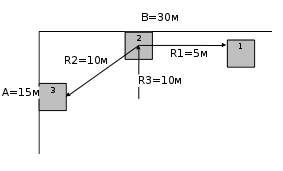
\includegraphics[width=0.6\textwidth]{noise}
\caption{Схема расположения расчетной точки относительно источников шума}
\label{pic:noises}
\end{figure}

Уровни звуковой мощности источников ($ L_p = f(f_{cr}) $) представлены в таблице~\ref{table:noise_lvl}.
Габаритные размеры помещения, $ A \times B \times C, м^3 $, $15 \times 30 \times 4$.
\begin{table}[bth]
\centering
    \begin{tabu}{|X[3,c]|X[1,c]|X[1,c]|X[1,c]|}
        \hline
        & Источник 1 & Источник 2 & Источник 3 \\
        \hline
        Уровень звуковой мощности & 9 & 1 & 8 \\
        \hline
    \end{tabu}
    \caption{Уровни звуковой мощности источников}
    \label{table:noise_lvl}
\end{table}

Объем помещения:
$$ V = A \cdot B \cdot C = 15 \cdot 30 \cdot 4 = 1800\ м^3 $$
Использумые обозначения:
\begin{itemize}
    \item $ \mu $ -- частотный множитель;
    \item $ \Phi = 1 $ -- фактор направленности источника шума;
    \item $ \chi = 1 $ -- коэффициент влияния ближнего акустического поля;
    \item $ y = 1 $ -- диффузность звукового поля в помещении.
\end{itemize}

Уровни интенсивности звука расчитываются по формуле:
$$ L_j = L_p + 10 \lg{(\frac{\Phi\chi}{S} + \frac{4y}{B})} $$

В таблице \ref{table:noise} представлены расчеты уровня звукового давления, а в таблице \ref{table:noise_intence}
представлены расчеты уровня звуковой интенсивности.

\begin{table}[bth]
\centering
    \begin{tabu}[\textwidth]{|X[5,c]|X[1,c]|X[1,c]|X[1,c]|X[1,c]|X[1,c]|X[1,c]|X[1,c]|X[1,c]|X[2,c]|}
        \hline
        Источник & \multicolumn{8}{c|}{Уровни звуковой мощности} & S \\
        \cline{2-9}
        & 63 & 125 & 250 & 500 & 1000 & 2000 & 4000 & 8000 & \\
        \hline
        \textnumero1, на полу, 5м & 90 & 91 & 98 & 99 & 97 & 93 & 91 & 86 & 157 \\
        \hline
        \textnumero2, подвешен, 10м & 84 & 82 & 84 & 91 & 94 & 94 & 91 & 91 & 314 \\
        \hline
        \textnumero3, на полу, 10м & 101 & 102 & 100 & 101 & 99 & 99 & 97 & 91 & 314 \\
        \hline
    \end{tabu}
    \caption{Параметры расчетов уровня звукового давления}
    \label{table:noise}
\end{table}

\begin{table}[bth]
\centering
    \begin{tabu}[\textwidth]{|X[3,c]|X[1,c]|X[1,c]|X[1,c]|X[1,c]|X[1,c]|X[1,c]|X[1,c]|X[1,c]|}
        \hline
        & \multicolumn{8}{c|}{Уровни звуковой интенсивности} \\
        \cline{2-9}
        & 63 & 125 & 250 & 500 & 1000 & 2000 & 4000 & 8000 \\
        \hline
        $Y$ & 0.8 & 0.75 & 0.7 & 0.8 & 1 & 1.4 & 1.8 & 2.5 \\
        \hline
        $B$ & 72 & 67.5 & 63 & 72 & 90 & 126 & 162 & 225 \\
        \hline
        Источник \textnumero1 & $ 77.919 $ & $ 79.171 $ & $ 86.442 $ & $ 86.919 $ & $ 84.060 $ & $ 78.811 $ & $ 75.922 $ & $ 69.829 $ \\
        \hline
        Источник \textnumero2 & $ 71.689 $ & $ 69.955 $ & $ 72.240 $ & $ 78.689 $ & $ 80.779 $ & $ 79.432 $ & $ 75.452 $ & $ 74.214 $ \\
        \hline
        Источник \textnumero3 & $ 88.689 $ & $ 89.955 $ & $ 88.240 $ & $ 88.689 $ & $ 85.779 $ & $ 84.432 $ & $ 81.452 $ & $ 74.214 $ \\
        \hline
        $ L_{max} $ & 83 & 74 & 68 & 63 & 60 & 57 & 55 & 54 \\
        \hline
        $ L_{j_{sum}} $ & 89.118 & 90.343 & 90.509 & 91.157 & 88.766 & 86.447 & 83.302 & 77.951 \\
        \hline
    \end{tabu}
    \caption{Параметры расчетов уровня звуковой интенсивности}
    \label{table:noise_intence}
\end{table}

Суммарный шум рассчитывается по следующей формуле:
$$ L_{j_{sum}} = 10\lg{(\sum_{i} 10^{\frac{L_i}{10}})} $$

\begin{figure}[bth]
\centering
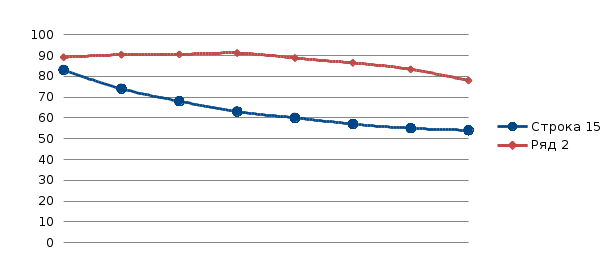
\includegraphics[width=0.8\textwidth]{noise_graph}
\caption{График распределения расчетного спектра уровня шума относительно предельно допустимых значений}
\label{pic:noise_graph}
\end{figure}

\subsubsection*{Выводы}
На рисунке \ref{pic:noise_graph} видно, что расчетный спектр превышает предельно допустимый уровень шума, причем на всех октавных частотах.
Замечено, что увеличение расстояния до источников шума довольно слабо влияет на его уровень.
Если изменить габариты помещения, то это может значительно повлиять на уровень шума в данном помещении в целом,
однако все равно не позволяет снизить его до допустимых значений. Рекомендованным защитным мероприятием в данном
случае будет являться акустическая обработка помещения, а также применение звукоизоляции.

\subsection{Расчет системы искусственного освещения}

С помощью программы DIALux были произведены расчеты, результаты которых представлены на рисунках \ref{pic:light_1},
\ref{pic:light_2}, \ref{pic:light_3}, \ref{pic:light_4} и \ref{pic:light_5}, при этом использовались
следующие параметры:
\begin{itemize}
    \item Габариты помещения: $ 7 \times 4 \times 2.8 $ (м);
    \item Коэффициенты отражения:
        \begin{itemize}
            \item Потолок: 31\% (медово-желтый цвет);
            \item Стены: 28\% (бежевый цвет);
            \item Пол: 18\% (Красно-оранжевый цвет);
        \end{itemize}
    \item Высота рабочей плоскости: 0.85 м;
    \item Планируемая освещенность: $ E = 300 лк. $
\end{itemize}

\begin{figure}[p]
\centering
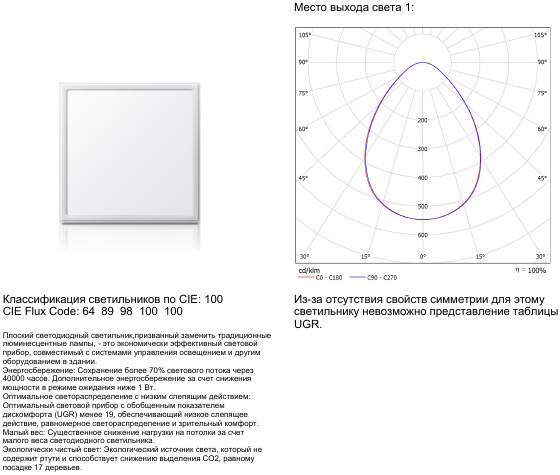
\includegraphics[width=\textwidth]{lights_1}
\caption{Паспорт светильника}
\label{pic:light_1}
\end{figure}
\begin{figure}[p]
\centering
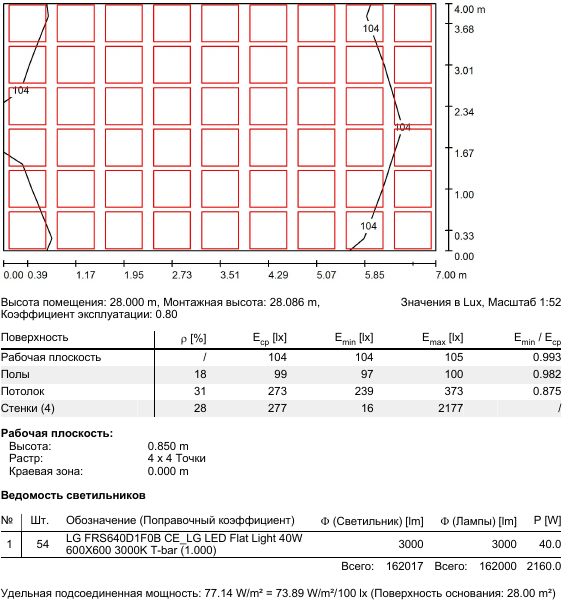
\includegraphics[width=\textwidth]{lights_2}
\caption{Резюме помещения}
\label{pic:light_2}
\end{figure}
\begin{figure}[p]
\centering
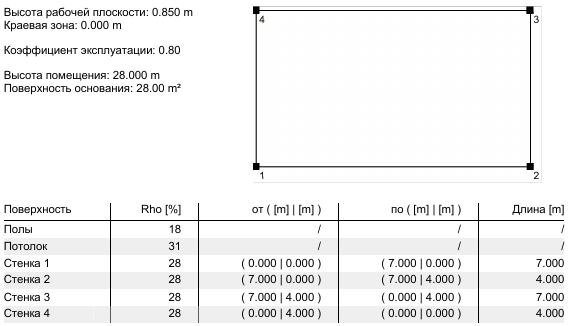
\includegraphics[width=\textwidth]{lights_3}
\caption{Протокол ввода помещения}
\label{pic:light_3}
\end{figure}
\begin{figure}[p]
\centering
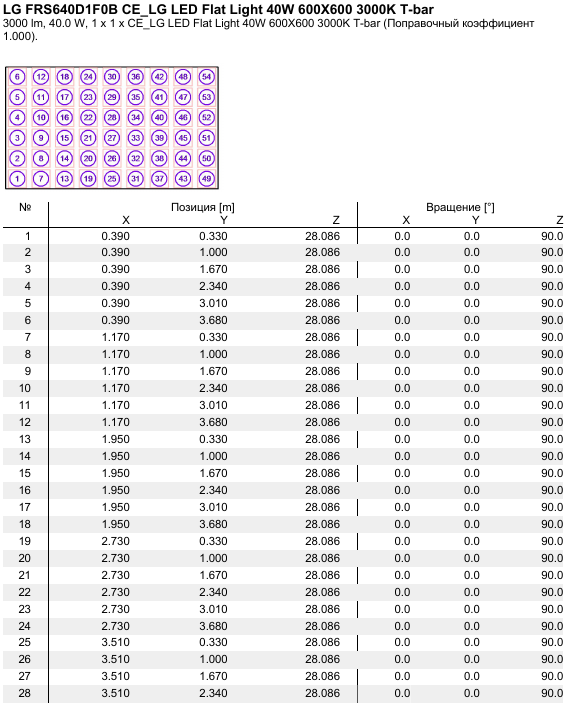
\includegraphics[width=\textwidth]{lights_4}
\caption{Светильники}
\label{pic:light_4}
\end{figure}
\begin{figure}[p]
\centering
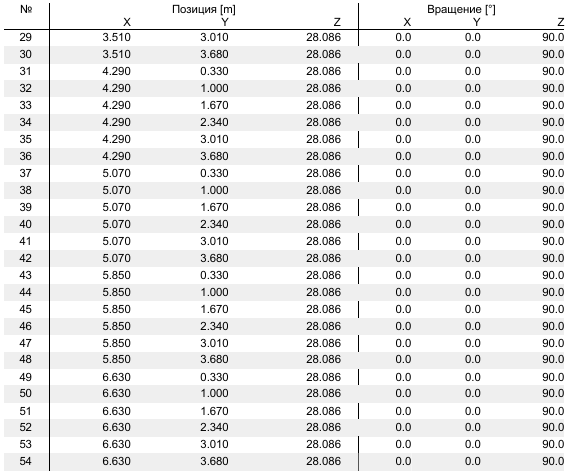
\includegraphics[width=\textwidth]{lights_5}
\caption{Светильники, список координат}
\label{pic:light_5}
\end{figure}
\clearpage
